\section{Introduction}
{\bf Our main story:

table extraction from the web has attracted a lot of attention, however, top-k extraction is more important, for the following reason:

\begin{itemize}
\item a lot of data. For table extraction, only Wikipedia table is useful
\item data is more clean
\item data has more semantics, with ranking info, typicality info, also include other columns (pictures, links, singers for songs, etc)
\item data is more interesting, people want to know top things
\end{itemize}
}


The world wide web is by far the largest source of information today.
Much of that information contains structured data such as tables and lists
which are very valuable for knowledge discoverage and data mining. 
This structured data is valuable not only because of the relational
values it contains, but also because it is relatively easier to unlock
information from data with some regular patterns than free text which
makes up most of the web content. However, when encoded in HTML, and 
interleaved with various HTML tags, structured data becomes 
``semi-structured''. And because HTML documents are often coded manually,
inconsistencies and errors are abundant in them. All these pose significant 
challenges in the extraction of structured data from the web.

In this paper, we focus on list data in web pages. In particular, we are 
interested in extracting from a kind of web pages that is {\em solely about}
a list of $k$ instances of a topic or a concept. Examples of such topic include 
``Top 10 Beaches in the World'', ``5 Hollywood Classics You Shouldn't Miss'', 
``50 tallest people in the world''. Figure \ref{fig:snapshotOfWebPage}
shows a snapshot of such a web page\cite{example1}.

\begin{figure}[h]
	\centering
	\includegraphics[width=8cm]{./pic/page5.eps}
	\caption{A {\em top-k page} snapshot}
	\label{fig:snapshotOfWebPage}
\end{figure}

Informally, our problem is to given a web page with a title that contains
a integer number $k$, check whether the page contains a list of $k$ items
as its main content, and if it does, extract these $k$ items. 
We call such lists {\em top-k lists} and pages that contain the 
entirety of a top-k list {\em top-k pages}.
There are also lists that span
multiple pages and are connected by hyperlinked ``Next'' button, such as
the page\cite{example2} shown in Figure \ref{fig:multipagelist}.
{\bf zzx: what about ``slideshow pages''?}
But this type of pages
are not considered in this paper. A typical scenario we consider, 
like the one in Figure \ref{fig:snapshotOfWebPage}, is that
each list item is more than an instance of the topic in the title, 
but instead contain additional information such as 
a textual description and images. Our objective
is to extract the actual instance whenever possible, but in the worst case,
produce list items that at least {\em contain} the wanted instances.

\begin{figure}[h]
	\centering
	\includegraphics[width=8cm]{./pic/page4.eps}
	\caption{A slideshow page snapshot}
	\label{fig:multipagelist}
\end{figure}

The work described in this paper is an important step in our bigger effort of
automatic constructing a universal knowledge base that includes large number 
of known concepts and their instances. To that end, we have already built one of
the largest open-domain taxonomy called Probase \cite{wentao} 
which consists of 2.7 million concepts and many more instances. 
However, that attempt primarily employs Hearst 
patterns \cite{Hearst92} to extract concept-instance pairs from web text, and
is unable to discover instances stored in structured web data such as
lists. Although there were previous attempts to extract lists from the web 
\cite{Lerman01:AutomaticData,LiuGZ03:MDR,MiaoTHSM09:TagPathClustering,
FumarolaWBMH11:HyLiEn}, 
these techniques can hardly solve our problem for three reasons.
First, these techniques focus on {\em deep web pages} 
which are generated by backstage servers and data bases. 
Thus, the list items in those pages are highly structured, 
which makes list extraction relatively easy.
When they turn to {\em top-k pages}, 
it becomes more complicated as they are mostly edited manually.
In fact, the effect of these methods reduce heavily when we use {\em top-k pages} as input.
Second, these techiques merely retrive all the lists in a page, 
and fail to decide which one to be the top-k list.
This is important for our problem 
because it is common for a {\em top-k page} to contain other lists 
like the lists showed in Figure \ref{fig:detailedWebPage} (d) and (e),
which is irrelavent to the topic of page.
Third, some of the techiques are not practicable for our problem,
because the algorithms behind them are so complicated and time-consuming,
that it may take too much time for analysing a single page.

{\bf zzx's words here.}

In addition to enriching the instance space of a knowledge base, the techniques
developed here can also be used in a fact look-up engine \cite{YinTL11:Facto}. 
If a user wants to find out who are the 10 tallest persons in the world, the 
engine could retrieve all pages with the terms ``10'' and ``tallest persons''
in their titles, use the techniques in this paper to extract 10
person names from each of the pages, and then combined the results to present
one high confidence list of persons using statistical methods.

The list extraction problem is challenging for the following reasons.
First we should make sure our solution to have a satisfied outcome, 
which is mainly indicated by the recall and precision value.
This requires our approach to handle most cases, including some ``tricky'' ones.
Second, we must offer a mechanism to value a few lists to pick up the right one
(or to filter the noise lists).
Third, it is not easy to get the exact name of the list items. For example, 
the exact name of the list item shown in Figure \ref{fig:detailedWebPage} (b) should be ``Seychelles''.
{\bf zzx's words here.}

This paper has the following contributions:
\begin{itemize}
\item We defined a novel top-k list extract problem which is useful in
knowledge discovery and fact answering (Section \ref{sec:problem});
\item We developed an unsupervised general-purpose algorithm that 
is capable of extracting top-k lists from any web pages 
(Section \ref{sec:algo});
\item Our evaluation shows that our algorithm scales with the data size
and achieves satisfactory accuracy (Section \ref{sec:eval}).
\end{itemize}
